%% chapter2_slides.tex
%% Beamer slides for Chapter 2: Validity -- E-values under the Null Hypothesis
%% "Hypothesis Testing with E-Values" by Aaditya Ramdas & Ruodu Wang (arXiv:2410.23614)
%% Reader-friendly style: complete sentences, symbol explanations, worked examples
%% Compiled with: pdflatex -interaction=nonstopmode chapter2_slides.tex  (twice)
\documentclass[aspectratio=169,10pt]{beamer}

\usetheme{Madrid}
\usecolortheme{seahorse}
\usefonttheme{professionalfonts}

%% ── Packages ──────────────────────────────────────────────────────────────
\usepackage{amsmath,amssymb,amsfonts}
\usepackage{mathtools}
\usepackage{graphicx}
\usepackage{booktabs}
\usepackage{xcolor}
\usepackage{listings}

\graphicspath{{figures/}}

%% ── Python listing style ─────────────────────────────────────────────────
\lstdefinestyle{pycode}{
  language=Python,
  basicstyle=\ttfamily\scriptsize,
  numbers=left,
  numberstyle=\tiny\color{gray},
  frame=single,
  backgroundcolor=\color{gray!7},
  keywordstyle=\color{blue!70!black}\bfseries,
  commentstyle=\color{green!50!black}\itshape,
  stringstyle=\color{orange!80!black},
  showstringspaces=false,
  breaklines=true,
  tabsize=4,
  xleftmargin=1.5em,
  framexleftmargin=1.5em,
  aboveskip=4pt,
  belowskip=4pt,
}

%% ── Metadata ─────────────────────────────────────────────────────────────
\title[E-Values -- Ch.2]{Hypothesis Testing with E-Values}
\subtitle{Chapter 2: Validity -- E-values under the Null}
\author{Based on Ramdas \& Wang}
\date{arXiv:2410.23614}

\setbeamertemplate{footline}[frame number]
\setbeamertemplate{navigation symbols}{}

%% Helpful macros
\newcommand{\PP}{\mathbb{P}}
\newcommand{\QQ}{\mathbb{Q}}
\newcommand{\EE}{\mathbb{E}}
\newcommand{\RR}{\mathbb{R}}
\newcommand{\calP}{\mathcal{P}}
\newcommand{\calQ}{\mathcal{Q}}
\newcommand{\calF}{\mathcal{F}}
\newcommand{\ind}[1]{\mathbf{1}_{\{#1\}}}

%% ══════════════════════════════════════════════════════════════════════════
\begin{document}

%% ── Title frame ──────────────────────────────────────────────────────────
\begin{frame}
  \titlepage
\end{frame}

%% ── Outline ──────────────────────────────────────────────────────────────
\begin{frame}{Chapter Overview}
  \tableofcontents
\end{frame}

\AtBeginSection[]{\begin{frame}{Outline}\tableofcontents[currentsection]\end{frame}}

%% ══════════════════════════════════════════════════════════════════════════
\section{Notation Recap}
%% ══════════════════════════════════════════════════════════════════════════

\begin{frame}[allowframebreaks]{Notation You'll Need / Recap}

This chapter studies what happens to e-values \emph{under the null hypothesis}
$\calP$ -- the alternative $\QQ$ never appears. Here is a compact,
self-contained recap: a one-slide refresher on the Chapter 1 basics, plus the
new ideas (calibrators, admissibility) that this chapter introduces.

  \begin{block}{Recap: e-variables, p-variables, and tests (from Chapter 1)}
    \begin{itemize}
      \item \textbf{Null hypothesis $\calP$}: a set of candidate probability
        distributions, one of which is assumed to be the ``true'' data-generating
        law if $H_0$ holds. Think of $\calP$ as ``all the ways the world could
        look if $H_0$ is true.''
      \item \textbf{E-variable (e-value) $E$ for $\calP$}: a nonnegative random
        variable with $\EE^\PP[E] \le 1$ for every $\PP \in \calP$. Intuition:
        a ``bet'' against $H_0$ that is fair or sub-fair on average whenever
        $H_0$ is true; a large realized value is evidence against $H_0$.
      \item \textbf{Exact e-variable}: one with $\EE^\PP[E] = 1$ for every
        $\PP \in \calP$ (no money left on the table, on average).
      \item \textbf{P-variable (p-value) $P$ for $\calP$}: a random variable
        with $\PP(P \le u) \le u$ for all $u \in [0,1]$ and all $\PP \in \calP$.
        Intuition: under $H_0$, $P$ is ``at least as spread out as uniform,''
        so small values of $P$ are surprising.
      \item \textbf{Exact p-variable}: $P$ is exactly $\mathrm{Uniform}[0,1]$
        under every $\PP \in \calP$.
      \item \textbf{Level-$\alpha$ test}: a $[0,1]$-valued random variable
        (a ``rejection probability'') whose $\PP$-expectation is at most
        $\alpha$ for all $\PP \in \calP$; a \emph{binary} test additionally only
        takes values in $\{0,1\}$ (reject / do not reject).
      \item $\PP \in \mathcal{M}_1$: shorthand for ``$\PP$ is a probability
        measure on the sample space,'' i.e., any legitimate candidate law.
    \end{itemize}
  \end{block}

  \framebreak

  \begin{block}{New in This Chapter}
    \begin{itemize}
      \item \textbf{Markov's inequality (for e-values)}: the classical bound
        $\PP(E \ge 1/\alpha) \le \alpha \EE^\PP[E]$, applied with
        $\EE^\PP[E]\le 1$. It is the single bridge connecting e-values to
        p-values and classical level-$\alpha$ testing.
      \item \textbf{Survival function $S(x;\PP) = \PP(E \ge x)$}: how likely
        $E$ is to be at least $x$, under a specific $\PP$. Knowing this exactly
        (rather than only its mean) lets us build sharper tests than Markov's
        inequality alone provides.
      \item \textbf{Calibrator}: a fixed, universal ``currency-exchange rule''
        that turns any p-value into a valid e-value (a \emph{p-to-e calibrator})
        or any e-value into a valid p-value (an \emph{e-to-p calibrator}), no
        matter which hypothesis or distribution produced it.
      \item \textbf{Domination / admissibility (calibrators)}: calibrator $f$
        dominates $g$ if $f$ always gives an equal-or-better exchange rate;
        $f$ is admissible if no other calibrator strictly beats it everywhere.
      \item \textbf{Admissible e-variable}: an e-variable that cannot be
        ``enlarged'' -- no other e-variable is always at least as big and
        sometimes strictly bigger. Intuition: it wastes no evidence.
      \item \textbf{Likelihood ratio}: for two candidate densities $p, q$, the
        ratio $q(Z)/p(Z)$; it is the prototypical (and, for simple nulls, the
        \emph{only}) admissible e-variable.
      \item \textbf{Pivotal e-variable}: one whose distribution
        $S(\cdot\,;\PP)$ does not depend on which $\PP \in \calP$ is true.
    \end{itemize}
  \end{block}

  \framebreak

  \begin{alertblock}{Running Example, Introduced Now}
    Throughout this deck we test the fairness of a coin: $H_0: \theta = 0.5$
    (probability of heads), based on $n=20$ independent flips, of which
    $x=14$ came up heads. We will compute an actual e-value, an actual
    p-value, and calibrate between them with real numbers at every stage.
  \end{alertblock}

\end{frame}

%% ══════════════════════════════════════════════════════════════════════════
\section{2.1 Testing using Markov's Inequality}
%% ══════════════════════════════════════════════════════════════════════════

\begin{frame}[allowframebreaks]{2.1 Testing Using Markov's Inequality}

E-values can already be interpreted as evidence against $H_0$ in their own
right. But it is natural to ask how an e-value can be converted -- perhaps
with some loss of efficiency -- into the more classical machinery of
level-$\alpha$ tests and p-values. The bridge is \textbf{Markov's inequality},
a two-line argument that turns \emph{any} e-value into \emph{any} desired test.

  \begin{block}{Proposition 2.1: Markov's Inequality for E-Values}
    Let $E$ be an e-variable for $\calP$. Then
    \[
      \PP(E \ge 1/\alpha) \le \alpha \quad \text{for all } \PP \in \calP,\ \alpha \in (0,1].
    \]
    Hence: $1/E$ is a p-variable; $(\alpha E) \wedge 1$ is a level-$\alpha$
    test; and $\ind{E \ge 1/\alpha}$ is a level-$\alpha$ binary test.
  \end{block}

  \begin{itemize}
    \item $E$: the e-variable, a nonnegative random quantity with
      $\EE^\PP[E]\le 1$ under $H_0$.
    \item $\alpha$: the significance level you choose in advance (e.g.\ 0.05).
    \item $1/\alpha$: the e-value threshold -- reject $H_0$ once $E$ crosses it.
    \item $x \wedge 1 := \min(x,1)$: clips a quantity at 1 so it is a valid
      ``rejection probability.''
    \item $\ind{A}$: the indicator, equal to 1 if event $A$ happens and 0 otherwise.
  \end{itemize}

  \framebreak

  \begin{block}{Proof of Proposition 2.1}
    \textbf{Step 1.} Start from the elementary inequality
    $\ind{x \ge 1} \le x$ for all $x \ge 0$ (a jump function is bounded by
    the identity line once you check $x<1$ and $x\ge1$ separately).

    \medskip
    \textbf{Step 2.} Substitute $x = \alpha E$:
    $\ind{\alpha E \ge 1} \le \alpha E$, i.e., $\ind{E \ge 1/\alpha} \le \alpha E$.

    \medskip
    \textbf{Step 3.} Take $\EE^\PP[\cdot]$ of both sides (expectation preserves
    $\le$):
    \[
      \PP(E \ge 1/\alpha) = \EE^\PP\big[\ind{E\ge 1/\alpha}\big]
      \le \alpha\, \EE^\PP[E] \le \alpha,
    \]
    using $\EE^\PP[E] \le 1$ in the last step (definition of e-variable). $\blacksquare$
  \end{block}

  \begin{alertblock}{Why This Is Conservative}
    Even though $1/E$ is technically a p-variable, it is usually a
    \emph{bad} one: it cannot be uniformly distributed on $[0,1]$ (so it is
    never exact), and it is typically far from it. Equality in Markov's
    inequality only occurs when $E$ is a two-point random variable
    supported on $\{0, 1/\alpha\}$ with mean 1 -- a very special case.
    In general, the type-I error of $\ind{E\ge1/\alpha}$ is strictly
    smaller than the nominal $\alpha$.
  \end{alertblock}

  \framebreak

  \begin{exampleblock}{Running Example: Applying Markov's Inequality to the Coin}
    We test $H_0:\theta=0.5$ using $n=20$ flips and observe $x=14$ heads.
    As our e-variable, take the likelihood ratio against the
    best-supported alternative $\theta_1 = x/n = 0.7$ (the maximum
    likelihood estimate):
    \[
      E = \frac{\theta_1^{\,x}(1-\theta_1)^{n-x}}{\theta_0^{\,x}(1-\theta_0)^{n-x}}
        = \frac{0.7^{14}\times 0.3^{6}}{0.5^{20}} \approx 5.18.
    \]
    (The binomial coefficient $\binom{n}{x}$ cancels between numerator and
    denominator.) This $E\approx 5.18$ is an exact e-variable for the simple
    null $\{\theta_0=0.5\}$ (Example 2.8 / Section 2.6.1 explain why).

    \medskip
    \textbf{Applying Proposition 2.1}: solving $1/\alpha = E$ gives
    $\alpha = 1/E \approx 0.193$. So the test ``reject if $E \ge 1/\alpha$''
    is only guaranteed level $\alpha\approx0.193$ here -- not very
    stringent, illustrating that Markov's inequality can be quite loose for
    a single, moderately-sized e-value.
  \end{exampleblock}

  \begin{block}{On the Book's Figure 2.2 (Redrawn Independently)}
    For the two-sided normal test of Chapter 1, comparing e-values (several
    $\delta$) against the classical p-value on a $\log_{10}$ scale shows that
    it is \emph{harder} for an e-value to reach 100 than for a p-value to
    reach 0.01 -- direct visual evidence that the Markov bound is generally
    conservative. See Figure~\ref{fig:normal} below (own redraw).
  \end{block}

  \begin{figure}
    \centering
    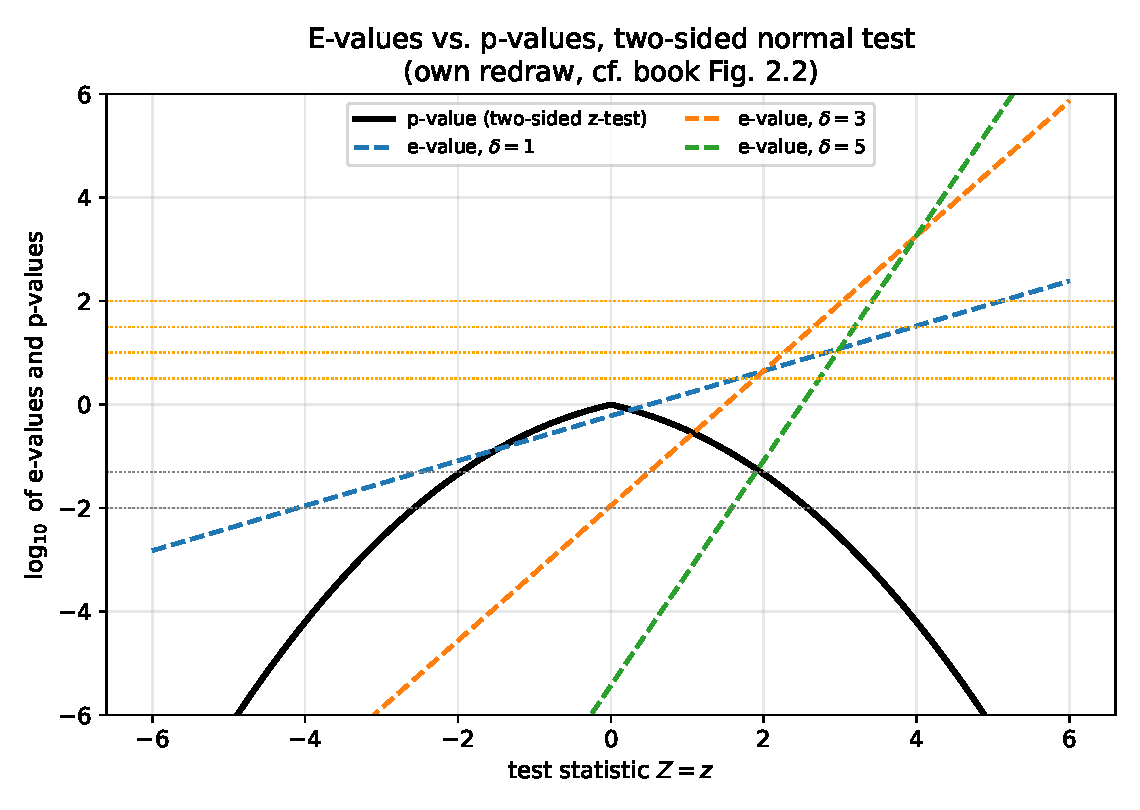
\includegraphics[width=0.62\linewidth]{fig4_evalue_pvalue_normal.pdf}
    \caption{E-values (for several $\delta$) vs.\ the p-value, two-sided
    normal test, as functions of the test statistic $Z$. \label{fig:normal}}
  \end{figure}

\end{frame}

\begin{frame}{Figure: Markov's Inequality, Simulated}
  \begin{columns}[T]
    \column{0.55\textwidth}
      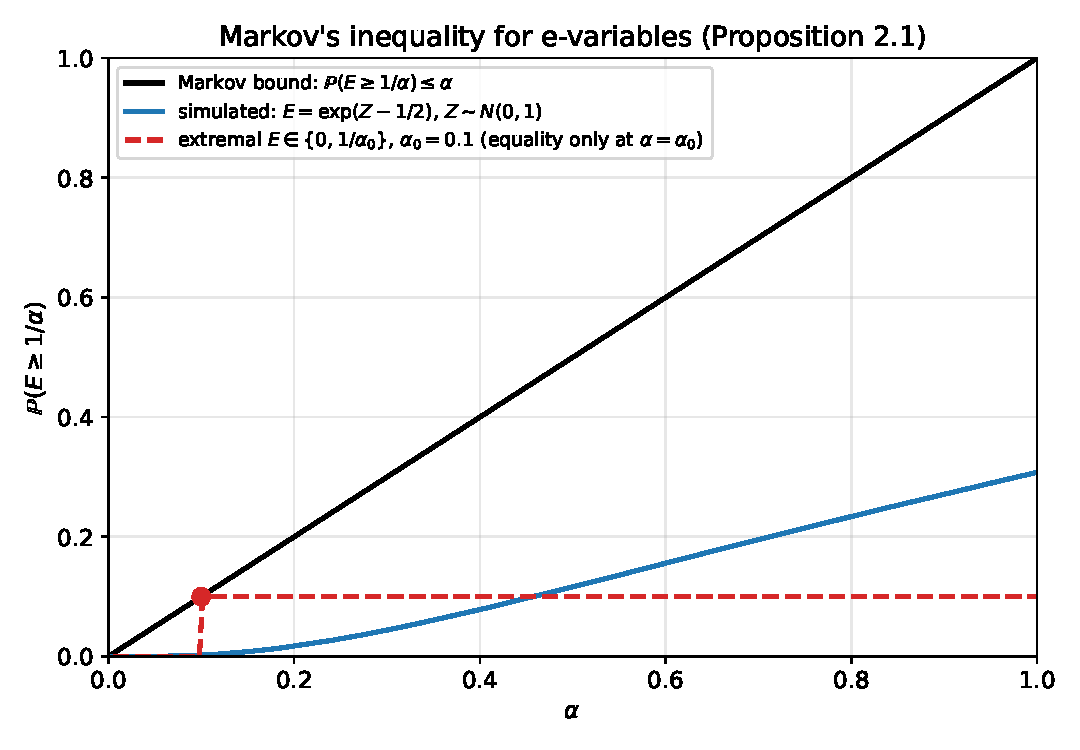
\includegraphics[width=\linewidth]{fig2_markov.pdf}
    \column{0.43\textwidth}
      \begin{block}{Reading the Plot}
        \begin{itemize}
          \item Black line: the Markov bound $\alpha \mapsto \alpha$ itself
            (an upper bound on $\PP(E\ge 1/\alpha)$).
          \item Blue curve: the \emph{actual} tail probability for a
            simulated exact e-variable $E=\exp(Z - 1/2)$, $Z\sim N(0,1)$ --
            always strictly below the bound (conservative).
          \item Red dashed: a two-point e-variable achieving
            \emph{equality} exactly at $\alpha_0=0.1$, the only case where
            Markov's inequality is tight.
        \end{itemize}
      \end{block}
  \end{columns}
\end{frame}

\begin{frame}[fragile]{Python: Markov's Inequality on the Coin Example}
\begin{lstlisting}[style=pycode]
import numpy as np
from math import comb

n, x = 20, 14                 # n flips, x heads observed
theta0, theta1 = 0.5, x / n   # null vs. MLE alternative

# Likelihood-ratio e-value for H0: theta = theta0
loglik = lambda th: x*np.log(th) + (n-x)*np.log(1-th)
E = np.exp(loglik(theta1) - loglik(theta0))
print(f"e-value E = {E:.4f}")               # E = 5.1844

# Markov's inequality: alpha = 1/E gives the guaranteed level
alpha_markov = 1 / E
print(f"Markov level alpha = 1/E = {alpha_markov:.4f}")  # 0.1929

# Monte Carlo check of Prop. 2.1 under the null: P(E >= 1/alpha) <= alpha
rng = np.random.default_rng(0)
sims = rng.binomial(n, theta0, size=2_000_000)
E_sim = np.exp(loglik(theta1) - loglik(theta0))  # same formula, vectorized below
def e_value(k):
    ll = lambda th: k*np.log(th) + (n-k)*np.log(1-th)
    return np.exp(ll(theta1) - ll(theta0))
E_all = e_value(sims)
alpha = 0.193
print("P(E >= 1/alpha) empirically:", np.mean(E_all >= 1/alpha), " <= alpha?", alpha)
\end{lstlisting}
\end{frame}

%% ══════════════════════════════════════════════════════════════════════════
\section{2.2 Testing using Distributional Knowledge}
%% ══════════════════════════════════════════════════════════════════════════

\begin{frame}[allowframebreaks]{2.2 Testing Using Distributional Knowledge}

Markov's inequality only uses the fact that $\EE^\PP[E]\le1$. If we actually
know (or can compute) the full distribution of $E$ under the null, we can
find sharper, smaller thresholds -- exactly as with any other classical test
statistic.

  \begin{block}{Survival Function}
    For an e-variable $E$ and $\PP \in \calP$, define the
    left-continuous survival function
    \[
      S(x;\PP) = \PP(E \ge x), \qquad x \in \RR.
    \]
    If $S(\cdot\,;\PP)$ is the same for every $\PP\in\calP$, we call $E$
    \textbf{pivotal} (its null distribution does not depend on which $\PP$
    in $\calP$ actually holds -- a very convenient property, revisited in
    Section 14.3).
  \end{block}

  \begin{itemize}
    \item $S(x;\PP)$: the chance, under a specific candidate law $\PP$, that
      the e-value is at least $x$. This is exactly the p-value you would
      report if you used $E$ itself (thresholded at $x$) as your test statistic.
    \item Pivotal: ``the same regardless of nuisance parameters within $H_0$.''
  \end{itemize}

  \begin{block}{Sharper Thresholds}
    For a threshold $t>0$, the test $\ind{E\ge t}$ has level $\alpha$ as soon
    as $\sup_{\PP\in\calP} S(t;\PP) \le \alpha$. Choosing $t\ge1/\alpha$
    always works (Markov), but we can typically do better. If
    $\PP\mapsto S(t;\PP)$ has a continuous supremum, the \emph{smallest}
    valid threshold is
    \[
      t^{*} = \inf\Big\{\, t>0 \;:\; \sup_{\PP\in\calP} S(t;\PP) \le \alpha \,\Big\}.
    \]
    This $t^{*}$ equals the largest left $\alpha$-quantile of $E$ over
    $\PP\in\calP$. When $\calP=\{\PP\}$ is simple, $t^{*}$ reduces to the
    plain left $\alpha$-quantile of $E$ under $\PP$.
  \end{block}

  \framebreak

  \begin{exampleblock}{Running Example: An Exact Threshold for the Coin}
    Reducing the threshold below $1/\alpha$ is just business as usual: treat
    $E$ as an ordinary test statistic. For our coin e-value $E$ (a function
    of $X=$ number of heads under $\theta_0=0.5$), we can compute the exact
    null distribution of $E$ by evaluating $E(k)$ for every
    $k=0,1,\ldots,20$, then read off the exact $\alpha$-quantile $t^{*}$
    directly from the (fully known, discrete) Binomial(20, 0.5) law --
    typically much smaller than the crude Markov threshold $1/\alpha$.
    This is exactly what the Python cell in Section 2.1 already computes
    when it enumerates \texttt{e\_value(k)} over all $k$.
  \end{exampleblock}

  \begin{alertblock}{Caveat}
    Even when $S(\cdot\,;\PP)$ is hard to pin down exactly, partial
    information about the distribution of $E$ can still yield useful bounds
    on $t^{*}$ that beat naive Markov -- this is developed further in
    Chapter 15.
  \end{alertblock}

\end{frame}

%% ══════════════════════════════════════════════════════════════════════════
\section{2.3 Relating P-Values and E-Values Using Calibrators}
%% ══════════════════════════════════════════════════════════════════════════

\begin{frame}[allowframebreaks]{2.3 Calibrators: Definitions}

P-values and e-values can be converted into each other via fixed,
universal ``currency-exchange'' functions called \textbf{calibrators}.
The key requirement is that the conversion must work \emph{for any}
hypothesis -- we are not allowed to peek at $\calP$ when designing $f$.

  \begin{block}{Definition 2.3: Calibrators}
    \begin{enumerate}
      \item[(i)] A \textbf{p-to-e calibrator} is a decreasing function
        $f:[0,\infty)\to[0,\infty]$ with $f=0$ on $(1,\infty)$, such that
        for \emph{any} hypothesis, $f(P)$ is an e-variable whenever $P$ is
        a p-variable.
      \item[(ii)] An \textbf{e-to-p calibrator} is a decreasing function
        $g:[0,\infty)\to[0,\infty)$ such that for any hypothesis, $g(E)$ is
        a p-variable whenever $E$ is an e-variable.
      \item[(iii)] Calibrator $f$ \textbf{dominates} $g$ if $f\ge g$
        (p-to-e case) or $f\le g$ (e-to-p case); domination is
        \textbf{strict} if further $f\ne g$. A calibrator is
        \textbf{admissible} if no other calibrator strictly dominates it.
      \end{enumerate}
  \end{block}

  \begin{itemize}
    \item Decreasing: bigger p-value (weaker evidence) $\Rightarrow$ smaller
      e-value, and vice versa -- calibrators must preserve the direction
      of evidence.
    \item $f=0$ on $(1,\infty)$: p-values larger than 1 do not occur, so we
      just define $f$ to vanish there for tidiness.
    \item Domination: ``$f$ never gives a worse exchange rate than $g$, and
      sometimes gives a strictly better one.''
    \item Admissible: the best you can do -- no other calibrator is
      uniformly at least as favorable.
    \item We often drop ``p-to-e'' and just say ``calibrator,'' because (as
      we will see) e-to-p calibrators turn out to be essentially unique.
    \item \textbf{Atomless} $\PP$: one under which some continuously
      distributed (e.g.\ uniform, normal) random variable exists. It
      suffices to verify calibrator properties on one atomless $\PP$.
    \end{itemize}

  \framebreak

  \begin{block}{Proposition 2.4: The Unique E-to-P Calibrator}
    The function $f(t)=\min(1,1/t)$ is an e-to-p calibrator. It dominates
    \emph{every} other e-to-p calibrator. In particular, it is the
    \emph{only} admissible e-to-p calibrator.
  \end{block}

  \begin{block}{Proof Sketch}
    \textbf{Step 1.} $f(t)=\min(1,1/t)$ is an e-to-p calibrator: this is
    exactly Markov's inequality (Proposition 2.1), giving
    $\PP(1/E \le u) \le u$ when $u=1/t$.

    \medskip
    \textbf{Step 2.} Suppose $g$ is another e-to-p calibrator with
    $g(t) < \min(1,1/t)$ for some $t$. Fix an atomless $\PP$. Two cases:
    (a) if $t>1$ and $g(t)<1/t$, build $E$ equal to $t$ with probability
    $1/t$ and $0$ otherwise -- then $g(E)$ fails to be a valid p-variable;
    (b) if $t\le1$ and $g(t)<1$, the deterministic e-variable $E=t$ shows
    $g(E)=g(t)<1$ is not uniform-dominated. Either way, $g$ cannot be a
    calibrator, a contradiction. So no calibrator can beat
    $\min(1,1/t)$ anywhere. $\blacksquare$
  \end{block}

  \framebreak

  \begin{block}{Proposition 2.5: Characterizing P-to-E Calibrators}
    A decreasing $f:[0,\infty)\to[0,\infty]$ with $f=0$ on $(1,\infty)$ is a
    p-to-e calibrator if and only if $\int_0^1 f(p)\,\mathrm{d}p \le 1$. It
    is \textbf{admissible} if and only if $f$ is upper semicontinuous
    (equivalently, left-continuous), $f(0)=\infty$, and
    $\int_0^1 f(p)\,\mathrm{d}p = 1$.
  \end{block}

  \begin{itemize}
    \item $\int_0^1 f(p)\,\mathrm{d}p$: the average value of $f$ applied to
      a Uniform$[0,1]$ random variable -- this must be at most 1 because
      $f(P)$ must itself be a valid e-variable (mean $\le 1$).
    \item $f(0)=\infty$: an admissible calibrator must reward a p-value of
      exactly 0 with infinite evidence -- otherwise it can be improved.
    \item Unlike the e-to-p direction, the class of admissible p-to-e
      calibrators is \emph{much richer} -- there is no single best choice.
  \end{itemize}

  \begin{block}{Proof Idea (``if'' direction)}
    \textbf{Step 1.} Since $f$ is decreasing and $P' \sim \mathrm{Uniform}[0,1]$
    stochastically dominates any p-variable $P$ (i.e.\ $\PP(P\le x)\le\PP(P'\le x)$),
    we get $\PP(f(P) > x) \le \PP(f(P') > x)$ for all $x$.

    \medskip
    \textbf{Step 2.} Integrating tail probabilities gives
    $\EE^\PP[f(P)] \le \EE^\PP[f(P')] = \int_0^1 f(p)\,\mathrm{d}p \le 1$,
    so $f(P)$ is indeed an e-variable. $\blacksquare$
  \end{block}

  \framebreak

  \begin{block}{A Menu of Admissible P-to-E Calibrators}
    \begin{align*}
      f(p) &= \kappa\, p^{\kappa-1} \quad \text{for some } \kappa\in(0,1)
             && \text{(power family, Eq.~2.1)}\\
      f(p) &= \int_0^1 \kappa p^{\kappa-1}\,\mathrm{d}\kappa
             = \frac{1-p+p\log p}{p(-\log p)^2}
             && \text{(mixture, Eq.~2.2)}\\
      f(p) &= 2(1-p) && \text{(Eq.~2.3)}\\
      f(p) &= p^{-1/2}-1 && \text{(Eq.~2.4)}\\
      f(p) &= -\log p && \text{(Eq.~2.5)}
    \end{align*}
  \end{block}

  \begin{itemize}
    \item $\kappa$ (kappa): a free tuning parameter trading off how much
      evidence very small $p$ gets versus moderate $p$.
    \item All five formulas above are admissible (Proposition 2.5): each
      integrates to exactly 1 over $p\in(0,1]$, is left-continuous, and
      blows up to $\infty$ as $p\to0$.
    \item Eqs.~2.3--2.5 penalize very small p-values \emph{less} steeply
      than Eq.~2.2, so they are less likely to manufacture huge e-values,
      but can be more useful when multiplying many independent e-values
      together.
  \end{itemize}

  \begin{figure}
    \centering
    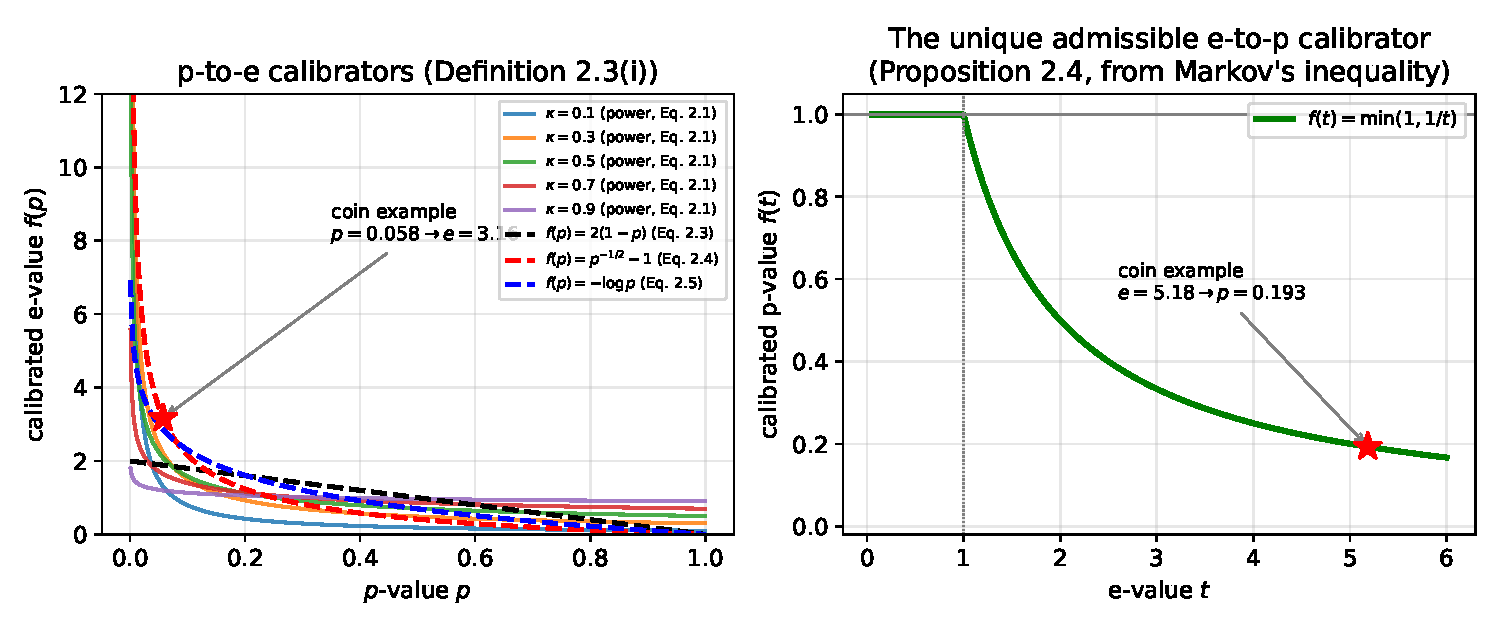
\includegraphics[width=0.85\linewidth]{fig1_calibrators.pdf}
    \caption{Left: several p-to-e calibrators, with the running coin
    example marked. Right: the unique admissible e-to-p calibrator
    $f(t)=\min(1,1/t)$, same example marked.}
  \end{figure}

  \framebreak

  \begin{exampleblock}{Running Example: Calibrating the Coin, Both Directions}
    Recall from Section 2.1: the coin data give a one-sided p-value
    $P \approx 0.0577$ (probability, under $\theta_0=0.5$, of 14 or more
    heads out of 20) and a likelihood-ratio e-value $E\approx 5.18$.

    \medskip
    \textbf{P-to-e, using Eq.~2.4}: $f(p)=p^{-1/2}-1$ gives
    \[
      f(0.0577) = 0.0577^{-1/2} - 1 \approx 4.164 - 1 = 3.16.
    \]
    This is a valid (if somewhat arbitrary) e-value manufactured purely
    from the p-value -- notably \emph{smaller} than the ``natural''
    likelihood-ratio e-value 5.18 computed directly from the model.

    \medskip
    \textbf{E-to-p, using Proposition 2.4}: $f(t)=\min(1,1/t)$ applied to
    $E\approx5.18$ gives
    \[
      \min(1, 1/5.18) \approx 0.193,
    \]
    a p-value much larger (more conservative) than the ``natural'' p-value
    $0.0577$ -- again showing the Markov conversion is lossy.
  \end{exampleblock}

  \framebreak

  \begin{alertblock}{A Warning: Do Not Round-Trip}
    Converting p $\to$ e $\to$ p (or e $\to$ p $\to$ e) generally loses a
    lot of evidence. Book example: starting from $p=0.01$, the calibrator
    $p\mapsto p^{-1/2}-1$ gives $e=9$; converting back with
    $e\mapsto\min(1/e,1)$ gives $p'=1/9\approx0.111$ -- eleven times
    weaker than the original $p=0.01$! \textbf{Moral}: calibrate once, in
    the direction you need, and stop.
  \end{alertblock}

  \begin{block}{Proposition 2.6 (Rescaling Calibrators)}
    If $f$ is a (admissible) calibrator, so is $x\mapsto a\,f(ax)$ for any
    $a\ge1$. \emph{Proof idea}: a change of variables shows the integral
    constraint $\int_0^1 g(x)\,\mathrm{d}x=1$ is preserved, and
    upper-semicontinuity / the value at 0 carry over directly from $f$.
  \end{block}

  \begin{block}{Proposition 2.7 (Every E-Variable Is a Calibrated P-Value)}
    Let $E$ be an e-variable for an atomless $\PP$. Then there exists a
    calibrator $f$ and an exact p-variable $P$ for $\PP$ such that
    $E=f(P)$ $\PP$-almost surely. If $E$ is exact, $f$ can be chosen
    admissible. \emph{Proof idea}: take $f$ to be (a version of) the
    right-quantile function of $E$; the standard quantile transform then
    produces an exact p-variable $P$ with $E=f(P)$.
  \end{block}

  \begin{exampleblock}{Example 2.8: The Two-Sided Normal Test}
    For $\PP=N(0,1)$ vs.\ $\QQ=N(\mu,1)$ with $n$ observations
    (Chapter 1's running example), the likelihood-ratio e-value is
    $E=\exp(\delta Z - \delta^2/2)$ and the Neyman--Pearson p-value is
    $P=\Phi(-Z)$, where $Z\sim N(0,1)$ under $\PP$, $\Phi$ is the standard
    normal CDF, and $\delta=\mu\sqrt{n}$. Both are exact, and indeed
    $E=f(P)$ with the admissible calibrator
    \[
      f(p) = \exp\!\big(-\delta\,\Phi^{-1}(p) - \delta^2/2\big).
    \]
  \end{exampleblock}

\end{frame}

\begin{frame}[fragile]{Python: Calibrating the Coin Example}
\begin{lstlisting}[style=pycode]
import numpy as np
from scipy import stats

n, x = 20, 14
theta0 = 0.5

# one-sided p-value: P(X >= 14) under Binomial(20, 0.5)
p_val = 1 - stats.binom.cdf(x - 1, n, theta0)
print(f"p-value = {p_val:.4f}")                 # 0.0577

# p-to-e calibrator, Eq. (2.4): f(p) = p^{-1/2} - 1
e_from_p = p_val ** (-0.5) - 1
print(f"calibrated e-value f(p) = {e_from_p:.3f}")   # 3.16

# natural likelihood-ratio e-value (theta1 = MLE = 0.7)
theta1 = x / n
loglik = lambda th: x*np.log(th) + (n-x)*np.log(1-th)
E_natural = np.exp(loglik(theta1) - loglik(theta0))
print(f"natural e-value = {E_natural:.3f}")          # 5.18

# e-to-p calibrator (Proposition 2.4): f(t) = min(1, 1/t)
p_from_e = min(1, 1 / E_natural)
print(f"calibrated p-value min(1,1/E) = {p_from_e:.3f}")  # 0.193

# Warning: round-tripping loses evidence -- verify with p=0.01
p0 = 0.01
e0 = p0 ** (-0.5) - 1               # 9.0
p0_back = min(1, 1 / e0)            # 0.111  (much weaker than 0.01!)
print(f"round-trip: p={p0} -> e={e0:.2f} -> p'={p0_back:.3f}")
\end{lstlisting}
\end{frame}

%% ══════════════════════════════════════════════════════════════════════════
\section{2.4 Randomized Tests and Calibrators}
%% ══════════════════════════════════════════════════════════════════════════

\begin{frame}[allowframebreaks]{2.4 Randomized Tests and Calibrators}

A \textbf{randomized test} uses independent external randomness (e.g., an
auxiliary coin flip you generate yourself) to sharpen a test. It turns out
external randomization can strictly improve Markov's inequality, giving a
strictly more powerful e-to-p calibrator.

  \begin{block}{Theorem 2.9: Randomized Markov Inequality}
    Fix $\PP\in\mathcal{M}_1$. Let $Y\ge0$ be a random variable and
    $U\sim \mathrm{Uniform}[0,1]$ independent of $Y$. Then for any $\alpha>0$,
    \[
      \PP(Y \ge U/\alpha) = \EE^\PP[\min(\alpha Y,1)] \le \alpha\,\EE^\PP[Y].
    \]
    In particular, if $Y$ is an e-variable for $\calP$, then
    $\PP(Y\ge U/\alpha)\le\alpha$ for all $\PP\in\calP$.
  \end{block}

  \begin{itemize}
    \item $U$: an independent auxiliary uniform random draw -- pure
      external randomness, generated by you, not by nature.
    \item Setting $U\equiv1$ recovers ordinary Markov's inequality
      exactly, so Theorem 2.9 strictly generalizes Proposition 2.1.
    \item If $Y$ is bounded, $Y\in[0,C]$ a.s., the inequality becomes an
      \emph{equality} for any $\alpha\le1/C$ -- randomization can make the
      bound tight in cases where plain Markov cannot.
    \end{itemize}

  \begin{block}{Proof}
    \textbf{Step 1.} Since $U$ is independent of $Y$ and uniform,
    conditioning on $Y$ gives $\PP(U\le \alpha Y \mid Y) = \min(\alpha Y,1)$.

    \medskip
    \textbf{Step 2.} Taking total expectation:
    $\PP(Y\ge U/\alpha) = \EE^\PP[\min(\alpha Y,1)] \le \alpha \EE^\PP[Y]$,
    using $\min(a,1)\le a$. $\blacksquare$
  \end{block}

  \framebreak

  \begin{block}{Corollary 2.10}
    For any hypothesis $\calP$: if a p-variable $P$ and an e-variable $E$
    are \emph{independent}, then $P/E$ is a p-variable. In particular, if
    $E$ is an e-variable, then $U/E$ is a p-variable, where
    $U\sim\mathrm{Uniform}[0,1]$ is independent of $E$.
  \end{block}

  \begin{alertblock}{Why Randomize?}
    Since $U<1$ almost surely, $U/E$ is a \emph{strictly smaller} (hence
    more powerful) p-value than $1/E$ in all but degenerate cases. The map
    $e\mapsto (U/e)\wedge1$ is itself an admissible \emph{randomized}
    e-to-p calibrator (Section 11.3) that dominates the non-randomized
    $e\mapsto(1/e)\wedge1$ -- the latter being admissible only \emph{among
    non-randomized} calibrators (Proposition 2.4).
  \end{alertblock}

  \begin{exampleblock}{Running Example: Randomizing the Coin Test}
    With $E\approx5.18$, draw an independent
    $U\sim\mathrm{Uniform}[0,1]$, say $u=0.4$ (a value you generate
    yourself, unrelated to the coin data). Then the randomized p-value is
    \[
      u/E \approx 0.4/5.18 \approx 0.077,
    \]
    smaller (more powerful) than the non-randomized $1/E\approx0.193$ from
    Section 2.3 -- though of course a \emph{different} draw of $U$ gives a
    different randomized p-value, which is the price of randomization.
  \end{exampleblock}

\end{frame}

%% ══════════════════════════════════════════════════════════════════════════
\section{2.5 Admissible E-Variables}
%% ══════════════════════════════════════════════════════════════════════════

\begin{frame}[allowframebreaks]{2.5 Admissible E-Variables}

Intuitively, an e-variable is \textbf{admissible} if it cannot be made
``bigger'' without breaking the e-variable property -- no evidence is left
on the table. This section characterizes admissibility precisely and
connects it to likelihood ratios.

  \begin{block}{Definition 2.11: Admissibility}
    An e-variable $E$ for $\calP$ is \textbf{admissible} if for any other
    e-variable $E'$ for $\calP$ with $E'\ge E$, we have $\PP(E'=E)=1$ for
    every $\PP\in\calP$. Equivalently: $E$ is admissible if it is not
    \textbf{dominated}, where $E'$ dominates $E$ means $E'\ge E$ always,
    and $\PP(E'>E)>0$ for some $\PP\in\calP$.
  \end{block}

  \begin{itemize}
    \item Domination: $E'$ is at least as large everywhere, and strictly
      larger with positive probability somewhere -- so $E'$ is a strict
      improvement on $E$.
    \item The constant $1$ is a (trivial) admissible e-variable for any
      $\calP$ -- it cannot be improved because any $E'\ge1$ dominating it
      would need $\EE^\PP[E']>1$ for some $\PP$, violating the e-variable
      constraint.
    \end{itemize}

  \begin{block}{2.5.1 Admissible E-Variables for a Simple Null Are Likelihood Ratios}
    \textbf{Proposition 2.12.} For a simple null $\{\PP\}$, an e-variable
    $E$ is admissible if and only if it is exact ($\EE^\PP[E]=1$). Further,
    every exact e-variable equals a likelihood ratio
    $\mathrm{d}\mathbb{S}/\mathrm{d}\PP$ almost surely, for some
    distribution $\mathbb{S} \ll \PP$ (absolutely continuous with respect
    to $\PP$).
  \end{block}

  \begin{itemize}
    \item $\mathrm{d}\mathbb{S}/\mathrm{d}\PP$: the likelihood ratio (Radon--Nikodym
      derivative) of a candidate ``evidence distribution'' $\mathbb{S}$ against
      the null $\PP$ -- exactly the classical statistical likelihood ratio.
    \item $\mathbb{S}\ll\PP$ (``$\mathbb{S}$ absolutely continuous with respect to
      $\PP$''): $\mathbb{S}$ assigns zero probability to every event that $\PP$
      assigns zero probability to, so the ratio is well defined.
  \end{itemize}

  \begin{block}{Proof Idea}
    \textbf{Step 1.} If $\EE^\PP[E]<1$, then $E+(1-\EE^\PP[E])$ is an
    e-variable strictly dominating $E$ -- so non-exact e-variables are
    never admissible.

    \medskip
    \textbf{Step 2.} Conversely, if $E'$ dominates an exact $E$, then
    $\EE^\PP[E']>1$, contradicting $E'$ being an e-variable -- so exact
    e-variables are always admissible.

    \medskip
    \textbf{Step 3.} Define $\mathbb{S}$ via
    $\mathrm{d}\mathbb{S}/\mathrm{d}\PP = E$; since $E\ge0$ is exact,
    $\mathbb{S}$ is a genuine probability measure absolutely continuous
    w.r.t.\ $\PP$. $\blacksquare$
  \end{block}

  \framebreak

  \begin{block}{2.5.2 Characterization of Admissibility (General $\calP$)}
    For $A\in\calF$ and $\delta>0$, write $\calP_A = \{\PP\in\calP:\PP(A)>0\}$
    and $\calP_A^\delta = \{\PP\in\calP:\PP(A)>\delta\}$.

    \medskip
    \textbf{Proposition 2.13 (necessary condition).} If $E$ is admissible
    for $\calP$, then for any $A\in\calF$ with $\calP_A\ne\varnothing$,
    $\sup_{\PP\in\calP_A}\EE^\PP[E]=1$.

    \medskip
    \textbf{Theorem 2.14 (full characterization).} $E:\Omega\to[0,\infty]$
    is an admissible e-variable for $\calP$ if and only if
    \[
      \liminf_{\delta\downarrow0}\ \inf_{\PP\in\calP_A^\delta}\
      \frac{1-\EE^\PP[E]}{\delta} = 0 \qquad \text{for all } A\in\calF.
    \]
  \end{block}

  \begin{itemize}
    \item $\calP_A$: the candidate laws that give event $A$ positive
      probability; $\calP_A^\delta$: those giving it probability above the
      threshold $\delta$.
    \item Theorem 2.14's condition says: for every event $A$, as we shrink
      the required probability $\delta$ of $A$ toward 0, we can always find
      candidate laws under which $E$ gets arbitrarily close to being exact
      \emph{relative to how much probability mass} $A$ carries.
  \end{itemize}

  \framebreak

  \begin{block}{Corollary 2.15: Easier Sufficient Conditions}
    An e-variable $E$ for $\calP$ is admissible if any one of:
    \begin{enumerate}
      \item[(a)] for each $A\in\calF$ with $\calP_A\ne\varnothing$, there
        exists $\PP\in\calP_A$ with $\EE^\PP[E]=1$ (\textbf{strong
        admissibility});
      \item[(b)] for each $\PP'\in\calP$, there exists $\PP\in\calP$ with
        $\PP'\ll\PP$ and $\EE^\PP[E]=1$;
      \item[(c)] $E$ is exact.
    \end{enumerate}
  \end{block}

  \begin{alertblock}{Strong Admissibility}
    Condition (a) is called \textbf{strong admissibility}. It is strictly
    stronger than plain admissibility in general (for infinite $\calP$, an
    admissible $E$ need not attain $\EE^\PP[E]=1$ for \emph{any} single
    $\PP$). But when $\calP$ is \textbf{finite}, Proposition 2.16 shows
    strong admissibility and admissibility \emph{coincide}.
  \end{alertblock}

  \framebreak

  \begin{block}{2.5.3 Admissible E-Variables on Product Spaces}
    Let $\calP'$ be probabilities on another space, and
    $\calP\times\calP' := \{\PP\times\PP' : \PP\in\calP,\PP'\in\calP'\}$.
    For $E$ on $\Omega$ and $E'$ on $\Omega'$, the product
    $E\times E'$ (defined by $(\omega,\omega')\mapsto E(\omega)E'(\omega')$)
    is an e-variable for $\calP\times\calP'$, because
    $\EE^{\PP\times\PP'}[E\times E'] = \EE^\PP[E]\,\EE^{\PP'}[E'] \le 1$.
  \end{block}

  \begin{block}{Proposition 2.17}
    If $E$ and $E'$ are \emph{strongly} admissible for $\calP$ and $\calP'$
    respectively, then $E\times E'$ is strongly admissible for
    $\calP\times\calP'$. \emph{(Proof idea: any product event $B$ contains
    a rectangle $A\times A'$ of positive product measure; apply strong
    admissibility of $E, E'$ on $A, A'$ separately and combine.)}
  \end{block}

  \begin{alertblock}{Practical Takeaway}
    Multiplying independent e-values for independent sub-problems (e.g.\
    $n$ i.i.d.\ coin flips, each contributing its own e-variable) preserves
    admissibility, as long as $\calP$ and $\calP'$ are finite (so strong
    admissibility applies via Proposition 2.16).
  \end{alertblock}

\end{frame}

\begin{frame}[fragile]{Python: Checking Admissibility on the Coin (Simple Null)}
\begin{lstlisting}[style=pycode]
import numpy as np

n, x = 20, 14
theta0 = 0.5

# For a SIMPLE null {theta0}, Prop. 2.12 says E is admissible
# iff it is EXACT, i.e. E_{theta0}[E] == 1.
def e_value_lr(k, theta1):
    loglik = lambda th: k*np.log(th) + (n-k)*np.log(1-th)
    return np.exp(loglik(theta1) - loglik(theta0))

theta1 = x / n   # 0.7, the MLE alternative used throughout this deck
k = np.arange(n + 1)
from scipy.stats import binom
pmf0 = binom.pmf(k, n, theta0)
E_k = e_value_lr(k, theta1)

mean_E = np.sum(pmf0 * E_k)
print(f"E_theta0[E] = {mean_E:.6f}")   # should equal 1.000000 (exact => admissible)

# Contrast: the mean-based e-variable from Sec. 2.6.3, (1-lam)+lam*Z/mu,
# lam=1, Z=heads, mu=10, is admissible via Corollary 2.15(b) despite NOT
# being exact in general (it is exact only at the boundary case Z=mu a.s.)
mu = n * theta0
Z = k
E_mean = Z / mu           # lambda = 1 special case
mean_E_mean = np.sum(pmf0 * E_mean)
print(f"E_theta0[Z/mu] = {mean_E_mean:.6f}")   # = 1.0 exactly for THIS theta0
\end{lstlisting}
\end{frame}

%% ══════════════════════════════════════════════════════════════════════════
\section{2.6 More Examples of E-Values}
%% ══════════════════════════════════════════════════════════════════════════

\begin{frame}[allowframebreaks]{2.6.1 Monotone Likelihood Ratio}

Many parametric families used in practice -- including the Binomial family
behind our coin example -- have the property that likelihood ratios are
monotone in the data. This lets us build e-variables for one-sided
hypotheses almost for free.

  \begin{block}{Proposition 2.18}
    Let $(\PP_\theta)_{\theta\in\Theta}$ have densities $(p_\theta)_{\theta}$
    with \textbf{monotone likelihood ratio}: for $\theta<\theta'$,
    $p_{\theta'}(z)/p_\theta(z)$ is increasing (or decreasing) in $z$.
    Consider testing $\calP=\{\PP_\theta:\theta\le\theta_0\}$ against
    $\calQ = \{\PP_\theta:\theta\ge\theta_1\}$, $\theta_1>\theta_0$. Then for
    any $\theta'>\theta_0$,
    \[
      E = \frac{p_{\theta'}(Z)}{p_{\theta_0}(Z)}
    \]
    is an e-variable for $\calP$.
  \end{block}

  \begin{itemize}
    \item Monotone likelihood ratio (MLR): larger data values $z$ favor
      larger $\theta$ -- a very common ``well-behaved'' pattern (satisfied
      by the Binomial, Normal, Poisson, and other exponential families).
    \item The claim covers our whole running example: $E\approx5.18$ from
      Section 2.1 is precisely an instance of Proposition 2.18 with
      $\theta_0=0.5$, $\theta'=\theta_1=0.7$, since the Binomial family has MLR.
    \end{itemize}

  \begin{block}{Proof Sketch (via Chebyshev's Association Inequality)}
    \textbf{Step 1.} Chebyshev's association inequality: for increasing
    $f,g$ and any random variable $X$,
    $\EE[f(X)g(X)] \ge \EE[f(X)]\EE[g(X)]$.

    \medskip
    \textbf{Step 2.} For $\theta\le\theta_0<\theta'$, write
    \[
      1 = \EE^{\theta_0}\!\Big[\tfrac{p_{\theta'}(Z)}{p_{\theta_0}(Z)}\Big]
        = \EE^{\theta}\!\Big[\tfrac{p_{\theta'}(Z)}{p_{\theta_0}(Z)}\cdot
                              \tfrac{p_{\theta_0}(Z)}{p_{\theta}(Z)}\Big]
        \ge \EE^{\theta}\!\Big[\tfrac{p_{\theta'}(Z)}{p_{\theta_0}(Z)}\Big]
            \EE^{\theta}\!\Big[\tfrac{p_{\theta_0}(Z)}{p_{\theta}(Z)}\Big]
        = \EE^{\theta}\!\Big[\tfrac{p_{\theta'}(Z)}{p_{\theta_0}(Z)}\Big],
    \]
    using Step 1's inequality (both ratios above are increasing in $z$
    under the MLR assumption) and $\EE^\theta[p_{\theta_0}(Z)/p_\theta(Z)]=1$
    (a change-of-measure identity). This gives $\EE^\theta[E]\le1$ for all
    $\theta\le\theta_0$, as required. $\blacksquare$
  \end{block}

  \begin{alertblock}{Optimality Preview}
    Section 6.7.1 will show this e-variable is actually \emph{log-optimal}
    against $\QQ=\PP_{\theta_1}$ -- simply because $p_{\theta_1}/p_{\theta_0}$
    is itself an e-variable for $\calP$, the best possible choice against
    that specific alternative.
  \end{alertblock}

\end{frame}

\begin{frame}[allowframebreaks]{2.6.2--2.6.7 Further Examples}

The book gives several more constructions of e-values for different testing
problems, several of which will recur (and be shown optimal) in later
chapters.

  \begin{block}{2.6.2 Testing Symmetry}
    $\calP = \{\PP: Z \stackrel{d}{=} -Z \text{ under } \PP\}$ (symmetric
    around 0). For a single observation with alternative density $q$, using
    $p^*(z)=\tfrac12(q(z)+q(-z))\ind{q(z)>0}$,
    \[
      E = \frac{2q(Z)}{q(Z)+q(-Z)}\ind{q(Z)>0}
    \]
    is an exact, admissible e-variable (Eq.~2.8). For $n$ i.i.d.\ symmetric
    data $X_1,\ldots,X_n$, natural families of e-variables include
    \[
      E_\lambda = \prod_{i=1}^n \frac{2\exp(\lambda X_i)}{\exp(\lambda X_i)+\exp(-\lambda X_i)},\qquad
      E_p = \frac{p^{k}(1-p)^{n-k}}{2^{-n}},
    \]
    where $k$ is the number of positive $X_i$'s (using that signs are i.i.d.\
    $\mathrm{Uniform}\{-1,1\}$ under $\calP$), plus signed-rank e-variables
    $E_\beta$ based on the Wilcoxon statistic.
  \end{block}

  \begin{block}{2.6.3 Testing the Mean (and Variance)}
    For nonnegative $Z$ and $\calP=\{\PP:\EE^\PP[Z]\le\mu\}$, both $1$ and
    $Z/\mu$ are e-variables, hence so is any mixture
    $(1-\lambda) + \lambda\, Z/\mu$, $\lambda\in[0,1]$ (Eq.~2.9) --
    admissible by Corollary 2.15(b) despite not being exact. Adding a
    variance bound $\mathrm{var}^\PP(Z)\le\sigma^2$ gives, via
    $\EE^\PP[Z^2]\le\mu^2+\sigma^2$, the further e-variable
    $(1-\lambda)+\lambda\,Z^2/(\mu^2+\sigma^2)$ (Eq.~2.10). For dependent
    data $(X_1,\ldots,X_n)$ with common marginal mean $\le\mu$,
    $(X_1+\cdots+X_n)/(n\mu)$ is an e-variable \emph{regardless of the
    dependence structure} -- no independence assumption needed at all.
  \end{block}

  \begin{exampleblock}{Running Example: The Mean-Based E-Variable for the Coin}
    View each flip as $X_i\in\{0,1\}$ with $\PP(X_i=1)=\theta$; under
    $H_0:\theta\le0.5$, the sum $Z=\sum_i X_i$ has mean at most
    $\mu = n\times0.5 = 10$. With observed $Z=14$, the e-variable
    $(1-\lambda)+\lambda Z/\mu$ is maximized at $\lambda=1$:
    \[
      E_{\text{mean}} = Z/\mu = 14/10 = 1.4.
    \]
    Compare to the parametric likelihood-ratio e-value $\approx5.18$ from
    Section 2.1: the distribution-free, mean-only e-variable is
    \emph{much weaker} evidence, illustrating the price paid for making
    fewer assumptions about the data-generating process.
  \end{exampleblock}

  \framebreak

  \begin{block}{2.6.4 Testing Sub-Gaussian Means}
    $\calP = \{\PP: \EE^\PP[e^{\lambda Z-\lambda^2/2}]\le1 \ \forall \lambda\ge0\}$
    (right tail lighter than a unit Gaussian, mean $\le0$). The family
    $\{e^{\lambda Z-\lambda^2/2}:\lambda\ge0\}$, and any mixture thereof,
    gives e-variables for $\calP$. A closely related null $\calP^0$
    (sub-Gaussian on \emph{both} tails, mean exactly 0) additionally admits
    $Z^2$ as an e-variable, because every $\PP\in\calP^0$ has variance
    $\le1$.
  \end{block}

  \begin{block}{2.6.5 Constrained Hypotheses}
    Generalizing 2.6.3--2.6.4: for a constraint set $\Psi\subseteq\mathcal{L}$
    (real measurable functions), define
    $\calP = \{\PP\in\mathcal{M}_1: \int f\,\mathrm{d}\PP\le0\ \forall f\in\Psi\}$
    (Eq.~2.13). For finite $\Psi=\{g_1,\ldots,g_K\}$, \emph{every} e-variable
    for $\calP$ is (quasi-surely) dominated by $1+\sum_{k=1}^K \pi_k g_k$ for
    some $\pi\in\RR_+^K$ -- a clean, complete description of all e-variables
    in terms of the defining constraints.
  \end{block}

  \begin{block}{2.6.6 Testing Likelihood Ratio Bounds}
    $\calP=\{\PP: \mathrm{d}\PP/\mathrm{d}\PP_0\le\gamma\}$ against
    $\QQ\ll\PP_0$ (closeness to a benchmark law $\PP_0$, in likelihood-ratio
    terms). The naive $E=(\mathrm{d}\QQ/\mathrm{d}\PP_0)/\gamma$ is an
    e-variable; it can be sharpened via quantile truncation to an improved
    e-variable $E^{*}\ge E$, using a classical risk-measure identity (Ch.~16).
  \end{block}

  \begin{block}{2.6.7 Testing Exchangeability}
    $\calP=\{\PP: Z\stackrel{d}{=}Z_\sigma\ \forall\sigma\in\mathcal{S}_n\}$,
    where $Z_\sigma$ permutes the $n$ coordinates. With $\pi$ a uniform
    random permutation independent of $Z$ and alternative density $q$,
    \[
      E = \frac{q(Z)}{\frac{1}{n!}\sum_{\sigma\in\mathcal{S}_n} q(Z_\sigma)}
    \]
    is an exact, admissible e-variable -- a ``soft-rank'' e-value (Section 1.7).
  \end{block}

\end{frame}

\begin{frame}[fragile]{Python: More E-Value Examples on the Coin}
\begin{lstlisting}[style=pycode]
import numpy as np
from scipy.stats import binom

n, x = 20, 14
theta0 = 0.5
mu = n * theta0                     # mean under H0: theta <= 0.5

# --- Sec. 2.6.3: distribution-free mean-based e-variable ---
lam = 1.0                            # best choice given Z > mu
E_mean = (1 - lam) + lam * x / mu
print(f"mean-based e-value (Z/mu) = {E_mean:.3f}")   # 1.400

# --- Sec. 2.6.1: parametric MLR-based e-value (theta1 = MLE) ---
theta1 = x / n
loglik = lambda th: x*np.log(th) + (n-x)*np.log(1-th)
E_lr = np.exp(loglik(theta1) - loglik(theta0))
print(f"likelihood-ratio e-value = {E_lr:.3f}")      # 5.184

# --- Sec. 2.6.2 flavor: symmetry-style e-value on the SIGNS of X_i-0.5 ---
# Reinterpret each flip's deviation sign S_i = sign(X_i - 0.5) in {-1,+1};
# under a fair coin the signs are i.i.d. Uniform{-1,1}, matching E_p below
# with p a candidate "bias" probability of a positive sign.
k = x                                 # number of "+1" signs = number of heads
p_cand = 0.7
E_signs = (p_cand**k * (1 - p_cand)**(n - k)) / (2**-n)
print(f"sign-based e-value at p={p_cand} = {E_signs:.3f}")

# Sanity check: E_lr and E_signs coincide here, since both reduce to the
# same binomial likelihood ratio construction.
\end{lstlisting}
\end{frame}

%% ══════════════════════════════════════════════════════════════════════════
\section{2.7 Informal Grids for Realized E-Values}
%% ══════════════════════════════════════════════════════════════════════════

\begin{frame}[allowframebreaks]{2.7 Informal Grids for Realized E-Values}

P-values are conventionally judged against thresholds like 0.01 or 0.05.
What is the analogous rule of thumb for e-values? Since e-values are
generalized likelihood ratios / Bayes factors, we can borrow Jeffreys's
classical grading scale for likelihood ratios.

  \begin{block}{Table 2.19: Jeffreys's Rule of Thumb, Applied to E-Values}
    \centering
    \begin{tabular}{lll}
      \toprule
      \textbf{e-value} & \textbf{level of evidence} & \textbf{Shafer's p-value} \\
      \midrule
      $[0,1)$        & null hypothesis is supported & $(0.25,1]$ \\
      $(1,3.16)$     & no more than a bare mention   & $(0.0577,0.25)$ \\
      $(3.16,10)$    & substantial                   & $(8.3{\times}10^{-3},0.0577)$ \\
      $(10,31.6)$    & strong                        & $(9.4{\times}10^{-4},8.3{\times}10^{-3})$ \\
      $(31.6,100)$   & very strong                   & $(9.8{\times}10^{-5},9.4{\times}10^{-4})$ \\
      $(100,\infty]$ & decisive                      & $[0,9.8{\times}10^{-5})$ \\
      \bottomrule
    \end{tabular}
  \end{block}

  \begin{itemize}
    \item ``Shafer's p-value'' column: the range of $p$ mapping to each
      e-value band under the calibrator $e=p^{-1/2}-1$ (Eq.~2.4), included
      purely for comparison -- it is \emph{not} a claim that e-values and
      p-values correspond one-to-one in general.
    \item These thresholds ($e>3.16$, $e>10$, etc.) work best for e-values
      obtained ``naturally'' (likelihood ratios or their generalizations),
      \textbf{not} for all-or-nothing e-variables like
      $E=\ind{P\le\alpha}/\alpha$, where $E=10$ is just $P\le0.1$ -- a very
      different notion of ``strength.''
  \end{itemize}

  \framebreak

  \begin{exampleblock}{Running Example: Grading Our Coin E-Value}
    Our natural likelihood-ratio e-value $E\approx5.18$ falls in the range
    $(3.16,10)$: \textbf{``substantial''} evidence against fairness by
    Jeffreys's scale -- consistent with (though not numerically identical
    to) the one-sided p-value $\approx0.058$, which sits just above the
    conventional 0.05 cutoff.
  \end{exampleblock}

  \begin{alertblock}{E-Values and P-Values Can Point in Different Directions!}
    A cautionary example (two-sided normal test, $Z\sim N(\mu,1)$): the
    classical p-value $P=1-\Phi(Z)$ does \emph{not} depend on which
    alternative $\delta=\mu$ you had in mind (it is uniformly most
    powerful), but the likelihood-ratio e-value
    $E=\exp(\delta Z-\delta^2/2)$ depends strongly on $\delta$. With
    $\delta=5$ and $Z=2$: $P\approx0.023$ (looks like evidence
    \emph{against} $H_0$), yet $E=\exp(10-12.5)=e^{-2.5}\approx0.082$
    (evidence \emph{for} $H_0$, since $E<1$)! \textbf{Lesson}: natural
    e-values and p-values need not agree in direction, because they encode
    different notions of evidence -- this is another reason not to compare
    them naively.
  \end{alertblock}

\end{frame}

%% ══════════════════════════════════════════════════════════════════════════
\section{Chapter Summary}
%% ══════════════════════════════════════════════════════════════════════════

\begin{frame}{Chapter 2 Summary}
  \begin{block}{What We Learned}
    \begin{itemize}
      \item \textbf{Markov's inequality} (Prop.\ 2.1) is the universal (if
        conservative) bridge from any e-value to a level-$\alpha$ test or
        p-value: $1/E$ is always a valid p-variable.
      \item Knowing the \textbf{exact null distribution} of $E$
        (Section 2.2) lets you use sharper thresholds than $1/\alpha$.
      \item \textbf{Calibrators} (Section 2.3) formalize the p-value
        $\leftrightarrow$ e-value exchange rate: the e-to-p direction has a
        \emph{unique} admissible calibrator $\min(1,1/t)$ (Markov's
        inequality again), while the p-to-e direction admits a rich family.
      \item \textbf{External randomization} (Section 2.4) strictly
        improves on Markov's inequality via Theorem 2.9.
      \item \textbf{Admissible e-variables} (Section 2.5) cannot be
        enlarged; for simple nulls they are exactly the likelihood ratios.
      \item Section 2.6 catalogued e-variables for monotone likelihood
        ratio families, symmetry, means/variances, sub-Gaussian means,
        constrained hypotheses, likelihood-ratio bounds, and exchangeability.
      \item Section 2.7's Jeffreys-style grid gives an informal way to
        interpret a realized e-value's strength -- but e-values and
        p-values need not even agree in \emph{direction}.
      \item \textbf{Running example}: our coin ($n=20$, 14 heads) yielded
        a likelihood-ratio e-value $\approx5.18$ (``substantial''
        evidence), a one-sided p-value $\approx0.058$, and we converted
        between them with real calibrators throughout.
    \end{itemize}
  \end{block}
\end{frame}

\end{document}
